\newgeometry{textwidth=16cm}
\chapter{Asphaltènes}
\minitoc
\restoregeometry

\newpage	
	\section*{Introduction}
	\spacing{1.5}
	
	Les enjeux de la compréhension des propriétés physiques et chimiques d'un système reposent sur l'arrangement des atomes qui constituent sa structure. Dans cette optique, chimistes et physiciens ont développé au cours des années diverses méthodes visant à caractériser les systèmes chimiques, en tenant compte de leur environnement. Ces avancées méthodologiques restent toutefois limitées par les moyens technologiques, et la modélisation des systèmes de grande dimension représente un défi de taille pour les chercheurs. Entrant dans cette catégorie, les asphaltènes demeurent des constituants mal connus du pétrole brut et leur nature exacte comme leur taille restent, aujourd'hui encore, autant de freins à la caractérisation précise, en termes de composition chimique, des huiles brutes. L'étude et la compréhension approfondie de ces systèmes représente pourtant un enjeu scientifique et économique majeur, la présence de ces composés dans toutes les étapes, de la production au raffinage du pétrole, impliquant à l'heure actuelle l'emploi de procédés spécifiques particulièrement onéreux \cite{akbarzadeh2007asphaltenes}. Plus précisément, les asphaltènes, présents sous forme de clusters ou de nanoparticules au sein des huiles brutes, tendent à augmenter la viscosité du pétrole brut et nécessitent des extractions chimiques successives, certaines étapes requérant de surcroît un traitement à haute température. \\
	
	Si les informations expérimentales (obtenues par spectrométrie de masse, pyrolyse, etc.) recueillies au fil des années sur les asphaltènes n'ont pas permis, à elles seules, d'élucider leur composition chimique ou leur arrangement, éléments clés qui ouvriraient la voie à une caractérisation approfondie, des études conjointes expérience-théorie ont révélé des éléments intéressants \cite{neurock1994molecular}. Notamment, l'étude des huiles lourdes en tant que systèmes biphasiques complexes requiert d'appréhender en premier lieu les phénomènes d'agrégation conduisant à la formation de micelles d'asphaltènes. L'organisation de ces micelles permet ensuite de mettre en lumière l'effet de l'addition de pentane, employé comme solvant dans l'extraction des asphaltènes.   \\
	
	
	En définitive, bien que la modélisation des asphaltènes sur la base de ces éléments ouvre des pistes à la compréhension des processus d'agrégation, de floculation et de précipitation de ces systèmes, il est devenu indispensable d'augmenter le niveau de précision des représentations chimiques des asphaltènes pour espérer comprendre leurs propriétés et prédire, sinon prévenir, les conséquences des phénomènes d'agrégation. 
	Dans cette optique, il convient de revenir à la composition moléculaire de base des asphaltènes. Les asphaltènes sont constitués d'un mélange hétérogène de structures polycondensées et d'hétéroatomes (azote, oxygène, soufre). La présence de ces hétéroélements induisant la formation de nombreuses interactions, notamment de type van der Waals, ces atomes constituent la clé de voûte de l'assemblage moléculaire \cite{zhang2013speciation, coelho2012elucidation}. Elucider les interactions intermoléculaires impliquant ces hétéroatomes est le premier enjeu dans la représentation approfondie de la structure des asphaltènes.  \\
	
	En reprenant l'ensemble des études réalisées jusqu'à ce jour sur la structure des asphaltènes, ce chapitre se veut un état des connaissances actuelles de ces systèmes. En pointant du doigt les zones d'ombre qui persistent dans la représentation de ces molécules, nous poserons le cadre de travail dans lequel s'inscrit la présente étude. 
	
	
	
	\newpage	
	
	\section{Définition}
	Historiquement, le premier emploi du terme "asphaltène" est attribué au français Boussingault, qui l'utilise dès 1837 pour caractériser certains des produits de distillation de l'asphalte \cite{goual2012petroleum}. Les "asphaltènes" sont alors les solides insolubles dans l'alcool mais solubles dans l'essence de térébenthine, par opposition aux "pétrolènes", constituants volatils solubles dans l'éther. \\
	A l'heure actuelle, le terme "asphaltène" désigne la fraction lourde du pétrole, insoluble dans les n-alcanes (tels que le n-pentane ou le n-heptane) mais soluble dans les solvants aromatiques tels que le toluène, la pyridine ou le benzène. D'un point de vue structural, les asphaltènes sont constitués de noyaux aromatiques condensés, substitués par des groupements aliphatiques et napthéniques et faisant intervenir des hétéroatomes (azote, soufre et oxygène) au sein d'arrangements de type hétérocycles \cite{strausz1992molecular}. La proportion globale d'hétéroatomes, comme la fraction précise d'atomes d'azote, de soufre ou d'oxygène, peut être quelque peu variable suivant les procédés d'extraction employés pour isoler les asphaltènes de l'huile brute \cite{calles2007properties}.
	
	\bigskip
	\section{Composition élémentaire}
	
	Les méthodes d'analyse principales appliquées pour déterminer la composition élémentaire d'une fraction lourde du pétrole ont été décrites par Barbelet \textit{et al.}\cite{barbelet1979analyses}. La composition élémentaire des asphaltènes en atomes de carbone et d'hydrogène semble varier faiblement suivant leur origine, et a été évaluée respectivement à $82\% \pm 3\%$ et $8.1\% \pm 0.7\%$ par Speight et Moschopedis \cite{speight1979some}. En outre, contrairement aux fractions plus légères du pétrole, au sein desquelles les hydrocarbures sont principalement de nature aliphatique (paraffine cyclique de type mono ou di-naphtène) ou monoaromatiques, les fractions lourdes incluent des structures naphténiques et aromatiques comportant plus de six cycles alkyliques.
	
	\subsection{Composition en hétéroatomes}
	
	
	\subsubsection{Soufre}
	Les dérivés soufrés contenus dans les asphaltènes sont semblables aux espèces que l'on retrouve dans les fractions plus légères du pétrole, mais leur proportion varie sensiblement. En règle générale, ces dérivés se divisent en cinq grandes classes chimiques : thiols, sulfures, disulfides, sulfoxydes et thiophènes. Thiols, sulfures, sulfoxydes et disulfides peuvent être classés plus précisément suivant leur nature cyclique ou acyclique, soit suivant l'organisation du squelette carboné (alkyle, aryle ou alkyl-aryle). Les dérivés thiophéniques, quant à eux, sont des structures polyaromatiques condensées autour d'un noyau thiophénique (benzo, dibenzo, naphtobenzo-thiophènes, etc.). Au sein des fractions lourdes, la majorité des espèces soufrées sont des dérivés thiophéniques, suivi par des dérivés sulfures (cycliques et acycliques). Des espèces de type sulfoxydes ont également pu être mises en évidence, dans des proportions très variables, leur teneur variant entre 0.3\% et 10.3\% \cite{merdrignac2007physicochemical, speight2004petroleum}.
	
	\subsubsection{Azote}
	Dans les fractions brutes, l'azote est présent en quantité inférieure aux autres hétéroéléments. On distingue néanmoins deux types de composés en fonction de la teneur en azote de l'asphaltène considéré. C'est ainsi que l'on distingue les composés "bases", dont la proportion d'azote est inférieure à l'unité, des composés "neutres". \\
	Les familles basiques qui ont pu être caractérisées présentent des structures dérivées de la quinoléine, contenant entre deux et quatre cycles aromatiques dont les configurations varient (péri ou catacondensées, avec différents degrés d'alkylation). Plus particulièrement, des benzo, dibenzo et tétrahydroquinoléines, ainsi que des azapyrènes ont été mis en évidence. \\ 
	De même, des structures neutres présentant divers degrés d'alkylation ont été détectées : carbazoles, benzo-carbazole et dibenzo-carbazoles. \\
	La proportion de structures neutres et basiques au sein d'une fraction brute est fortement liée aux paramètres géochimiques du site de provenance du pétrole. 
	Enfin, il est à noter que des structures dérivées de la porphyrine ont été mises en évidence, même si de tels composés se retrouvent en proportions plus anecdotiques. Leur présence, caractérisée au travers du complexe qu'elles ont tendance à former avec les ions nickel ou vanadium, dépend une fois de plus de l'origine du pétrole dont est extraite la fraction lourde. Le pourcentage d'occurence de ces structures varie communément entre 0.6 et 3.3\% \cite{merdrignac2007physicochemical, speight2004petroleum}.
	
	\subsubsection{Oxygène}
	Des structures oxygénées se retrouvent également dans les fractions lourdes du pétrole, leur teneur variant entre 0.3\% et 4.9\% \cite{speight2004petroleum}. Différentes familles ont pu être identifiées, notamment des dérivés du phénol, tandis que la caractérisation de groupements carboxyles révèle la présence d'ester, d'acides carboxyliques, de cétones, d'amides ou de sulfoxydes.
	
	
	\bigskip
	
	\section{Poids moléculaire des asphaltènes}
	
	Un rapide passage en revue de la bibliographie des asphaltènes révèle tout le débat autour de leur poids moléculaire. En effet, la distribution, en termes de poids moléculaire, varie entre 400 et 1500 Da pour les fractions de faible poids moléculaire, et peut atteindre $10^{6}$ Da pour les fractions de haut poids moléculaire \cite{mullins2008contrasting}. Le phénomène d'agrégation des asphaltènes est une des raisons avancées pour justifier qu'a l'heure actuelle aucune méthode n'ait permis de déterminer avec précision le véritable poids moléculaire de ces espèces. De nombreux procédés ont été employés pour tenter de résoudre ce problème, mais ceux-ci conduisent à des résultats ambigüs, qu'il serait hasardeux de généraliser. A titre d'exemple, des mesures par osméométrie à tension de vapeur font apparaître des résultats fortement dépendants du type de solvant employé ; en présence d'un solvant apolaire tel que le toluène, les résultats apparaissent surestimés, au contraire de l'utilisation d'un solvant polaire telle que la pyridine ou le nitrobenzène. 
	%S'agissant d'autres méthodes d'analyse, Groenzin et Mullins\cite{groenzin2000molecular} parviennent, par spectroscopie de fluorescence résolue en temps, à un poids moléculaire moyen de 750 Da environ, pour une distribution de 500 à 1000 Da, là où Pinkston et col.\cite{pinkston2009analysis} rapportent une distribution de 350 à 1050 Da pour une étude par spectrométrie de masse de résonance cyclotronique ionique à transformée de Fourier (FT-ICR). Ces derniers supposent l'existence de fragments de plus bas poids moléculaires, non détectés même à haute énergie électronique du fait de la stabilisation des intermédiaire obtenus par les chaînes alkyles des asphaltènes. 
	
	
	Merdrignac et col.\cite{merdrignac2006evolution} rapportent l'évolution du poids moléculaire des asphaltènes et comparer les changements causés par le procédé d'hydroconvertion. 
	
	\bigskip
	
	
	\section{Caractérisation de la structure moléculaire des asphaltènes}
	
	%\subsection{Modèles structuraux }
	
	La description de la structure des asphaltènes repose à l'heure actuelle sur deux modèles construits sur la base des résultats de diverses caractérisations expérimentales.  
	Le premier modèle, baptisé "modèle continental", représente les asphaltènes comme de larges coeurs constitués de quatre à dix cycles aromatiques condensés, ramifiés par des chaînes alkyles courtes \cite{groenzin2000molecular}. Ce modèle a été proposé par Zhao \textit{et al.} \cite{zhao2001molecular}figure\ref{figZ1} après caractérisation des asphaltènes obtenus par fractionnement avec du pentane supercritique, puis remployé par Rogel et Carbognani \cite{rogel2003density} dans leur travail sur des asphaltènes stables et instables extraits de pétrole provenant du Vénézuela. 
	Ce type de représentations est corrélé par des analyses en spectroscopie RMN, diffraction des rayons X et spectroscopie de fluorescence résolue en temps (TRDF). 
	
	
	
	\begin{figure}
		\centering
		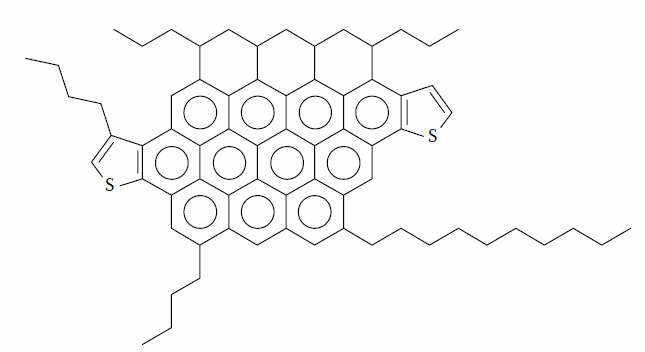
\includegraphics[scale=0.8]{image/Zhao}
		\caption[Structure moyenne du modèle continental des asphaltènes]{Structure moyenne du modèle continental des asphaltènes. Zhao et col. 2001}
		\label{figZ1}
	\end{figure}
	
	
	Le modèle "archipel" présente quant à lui ces systèmes comme un ensemble de régions à caractère aromatique, constituées de deux à trois cycles condensés, reliées par des chaînes carbonées. Ce modèle s'appuie sur des analyses par pyrolyse, oxydation, dégradation thermique et dispersion angulaire neutronique, telles que rapportées par Gawrys \textit{et al.} \cite{gawrys2003role}. Sheremata \textit{et al.}\cite{sheremata2004quantitative} ont notamment employé ce modèle pour la description des asphaltènes, comme le présente la figure reproduite ci-dessous (figure \ref{fig2}). 
	
	\begin{figure}
		\centering
		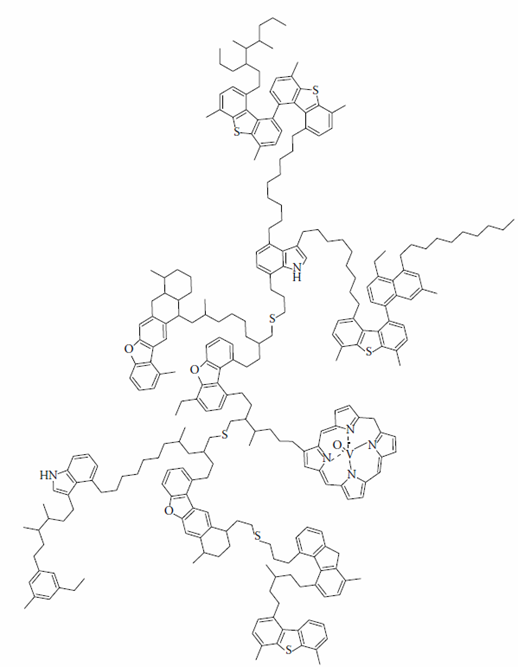
\includegraphics[scale=0.8]{image/Sher}
		\caption[Molecule d'asphaltènes type archipel]{Représentation d'asphaltènes à l'aide du modèle archipel, proposé par Sheramata \textit{et al.}}
		\label{fig2}
	\end{figure}
	
	Ces deux modèles, basés sur des structures moléculaires bien distinctes, conduisent néanmoins à des propriétés physico-chimiques différentes. La description des agrégats d'asphaltènes ainsi que leur solubilité dans le pétrole brut seront nettement impactées par l'emploi de l'un ou l'autre de ces modèles. Du fait de la planéité induite par la présence d'un grand nombre de cycles aromatiques condensés, la représentation d'un agrégat d'asphaltènes dans le cadre du modèle continental conduit à un empilement de plans. A l'inverse, les chaînes alkyles du modèle archipel confère une toute autre géométrie à ces systèmes : les asphaltènes peuvent se courber par le biais d'interactions moléculaires pour former des macro-agrégats globulaires susceptibles de piéger les molécules de solvant. 
	
	
	
	\subsection{Analyses par spectroscopie RMN}
	
	La spectroscopie de résonance magnétique nucléaire est couramment employée pour l'analyse structurale et la caractérisation de matériaux et de substances organiques. 
	%Elle est fondée sur les propriétés magnétiques de certains noyaux atomiques.Les noyaux les plus étudiés, dans le cadre de la chimie organique sont l'hydrogène $^{1}H$ et le carbone $^{13}C$. 
	Cette technique représente donc une méthode d'analyse de choix pour l'étude des asphaltènes et a, à ce titre, permis d'acquérir les premiers résultats visant à résoudre leur composition chimique. Dès 1982, les travaux de Murphy \textit{et al.} \cite{murphy1982determination} révèlent que la structure primaire des asphaltènes se compose de multiples cycles aromatiques condensés (l'indice de condensation relevé sur ces systèmes étant de 3 au moins) ainsi que d'une grande variété de chaînes aliphatiques, longues et ramifiées. Par la suite, les travaux de Yen \textit{et al.} en RMN $^{1}H$ ont donné une première idée de la proportion d'hydrocarbures saturés en regard de la fraction d'hydrocarbures aromatiques au sein de molécules d'asphaltènes  \cite{yen1984study}. Enfin, plus récemment, Durand \textit{et al.} ont employé les résultats de leurs analyses par RMN $^{13}C$ pour évaluer les indices de substitution et de condensation d'échantillons d'asphaltènes de différentes origines \cite{durand2010effect}. Leur étude tend à démontrer qu'au sein d'agrégats d'asphaltènes cohabitent les deux modèles structuraux évoqués ci-avant, à savoir le modèle continental et le modèle archipel. 
	
	
	\subsection{Analyses par diffraction des rayons X}  
	
	Une étude du caractère aromatique et des paramètres cristallins des asphaltènes, des résines et des gilsonites issus du pétrole a été présentée par Yen \textit{et al.} sur la base d'analyses par diffraction des rayons X \cite{yen1961investigation}. Leurs résultats, confortés par les travaux réalisés par Shirokoff \textit{et al.} sur quatre échantillons d'asphaltènes issus d'huiles brutes provenant d'Arabie Saoudite \cite{shirokoff1997characterization}, représentent les asphaltènes comme des feuillets de cycles aromatiques condensés portant des ramifications de natures naphténiques et aromatiques.
	Toutefois, Altget et Boduszynky rappellent judicieusement dans leur étude \cite{altgeltcomposition} qu'il convient de prendre avec précaution les résultats provenant d'analyses en diffraction, lorsque les données géométriques fournies par l'analyse servent de base pour construire un modèle structural du système étudié. Leurs travaux semblent en outre indiquer que la détermination du caractère aromatique des asphaltènes est, par ce biais, inappropriée sinon arbitraire. 
	
	
	
	\subsection{Analyses par spectroscopie de Fluorescence Résolue en Temps} 
	
	Cette méthode d'analyse a été employée à plusieurs reprises pour tenter d'élucider plus précisément la taille et la structure de molécules d'asphaltènes faiblement agrégées.  
	Les premiers travaux en ce sens, réalisés par Groenzin et Mullins  \cite{groenzin1999asphaltene}, tendent à montrer que les molécules d'asphaltènes ne seraient constituées que d'un seul groupe chromosphère. En effet, le faible poids moléculaire obtenu pour ces systèmes, comme la coloration des molécules, sont autant d'éléments recueillis incompatibles avec la représentation des asphaltènes sous forme de larges structures pseudo-polymériques constitués de deux ou trois cycles aromatiques reliés entre eux par de longues chaînes aliphatiques. En définitive, ces premières analyses semblent conforter la représentation des asphaltènes par le modèle continental. \\
	Par la suite, Souza \textit{et al.} ont rapporté l'agrégation persistante des asphaltènes à la faible concentration de 0.8 g/L, soit sous le seuil de concentration critique de nanoagrégation \cite{souza2009study}. Leurs travaux corroborent par ailleurs les résultats de Groenzin \textit{et al.} quant à la structure des molécules d'asphaltènes en cela qu'ils concluent à une structure primaire constituée par un anneau polyaromatique de quatre cycles ou plus. 
	
	
	\bigskip
	
	\subsection{Analyses par spectroscopie infrarouge}
	
	La caractérisation d'un système chimique en termes de composition passe nécessairement par des analyses en spectroscopie infrarouge, laquelle permet l'identification des groupements fonctionnels de ce système. Toutefois, l'étude des fractions lourdes du pétrole, la diversité chimique et la taille des espèces présentes rend complexe l'utilisation de la spectroscopie IR. C'est ce que soulignent Yuan \textit{et al.}, qui relèvent l'existence d'un faible nombre d'analyses employant l'infrarouge moyen pour la caractérisation physique et chimique des huiles lourdes \cite{hongfu2006determination}. 
	Parmi les travaux notables, l'étude couplée en spectroscopies IR et UV-sisible menée par El-Bassoussi \textit{et al.} sur deux échantillons d'asphaltènes provenant d'Egypte a permis de classifier les espèces présentes en mono, di et polyaromatiques. En accord avec les deux modèles de représentation des asphaltènes, les espèces prédominantes sont les espèces di ou polyaromatiques \cite{el2010characterization}. En 2007, Rodrigues Coelho \textit{et al.} \cite{coelho2007characterization} démontrent l'existence d'une corrélation linéaire entre les intensités des bandes infrarouges symétriques et antisymétriques associées aux atomes d'hydrogène aromatiques de type arènes méthyl-substitués dans les régions 2900-3100 $cm^{-1}$ et 700-900 $cm^{-1}$. Enfin, Laxalde \textit{et al.} \cite{laxalde2014combining} rapportent une interprétation ajustée sur les structures modèles des asphaltènes en repérant les vibrations de stretching des liaisons C-H (hors du plan) et C=C.
	
	\bigskip
	
	\section{Coexistence des structures moleculaires}
	
	La compilation de l'ensemble de ces résultats expérimentaux tend à suggérer que les deux modèles structuraux des asphaltènes peuvent coexister au sein des fractions lourdes. Cette idée est appuyée par les résultats d'Acevedo \textit{et al.} \cite{acevedo2004structural, gutierrez2001fractionation} qui ont montré que les asphaltènes pouvaient se diviser en deux fractions : une fraction insoluble dans le toluène, baptisée A1, qui serait rigide et plane, conformément au modèle continental, et une fraction soluble dans le toluène grace à de nombreuses interactions intermoléculaires, baptisée A2 et qui correspondrait au modèle archipel. Sur la base de ces éléments, Acevedo et son équipe ont mis en place une nouvelle représentation des agrégats d'asphaltènes. Le système colloïdal consisterait en une fraction d'asphaltènes A1, entourés par une couche d'asphaltènes A2, ces derniers aidant à la solubilisation de l'ensemble. 
	En définitive, une revue bibliographique des analyses menées à ce jour sur les asphaltènes montre qu'aucun modèle structural définitif n'a pu être validé pour ce type de systèmes. De nombreux travaux cherchent encore à clarifier l'architecture moléculaire des asphaltènes, à deux échelles distinctes. En premier lieu, l'étude de la microstructure correspond à des systèmes de poids moléculaires variant entre 500 et 10 000 Da, soit à des nano-agrégats d'asphaltènes. En second lieu, les travaux sur la macrostructure de ces entités correspondent à l'étude d'assemblages de ces nano-agrégats d'asphaltènes et sont intimement liés au milieu. 
	
	
	\bigskip
	
	\section{Construction de la structure moléculaire des asphaltènes}
	
	La construction d'un modèle moléculaire utilisable en simulation se fait sur la bases des données expérimentales recueillies, suivant deux méthodes principales. 
	La première méthode repose sur une corrélation des résultats empiriques utilisés pour déduire des informations structurales. Dans le cas des asphaltènes, l'existence de nombreux cycles aromatiques et l'ensemble des données obtenues concernant la longueur des chaînes aliphatiques ont permis à Takanohashi \textit{et al.} d'étudier trois structures distinctes d'asphaltènes générées par la méthode de Sato par le biais de simulation en dynamique moléculaire \cite{takanohashi2004structural}. 
	La seconde méthode consiste à identifier des caractéristiques structurales propres au système ainsi que sa composition moléculaire en suivant un processus stochastique. Le modèle structural se construit par l'addition des données expérimentales et/ou par recoupement de ces résultats avec une base de données existantes. Cette méthode a été poursuivie aussi bien par Elyashberg \textit{et al.} \cite{elyashberg2008computer}, qui ont développé un algorithme permettant la construction d'une structure sur la base de données RMN, que par Todeschini \textit{et al.} \cite{todeschini1995weighted} qui ont quant à eux employé des propriétés physiques telles que l'hydrophobie, le point de fusion et le point d'ébullition. 
	La construction d'un modèle moléculaire des asphaltènes peut en dernier lieu se faire initialement de façon plus intuitive, les informations expérimentales servant ensuite à optimiser le modèle de départ \cite{faulon1996stochastic,al2012systematic,de2012monte}. 
	
	
	
	\bigskip
	
	\section{Modélisation moléculaire des asphaltènes}
	
	La chimie computationnelle a révolutionné notre façon d'appréhender la structure et la réactivité des molécules, de sorte que la simulation est désormais une des clés de voûte de l'avancée scientifique. 
	Comme nous l'avons souligné dans les paragraphes précédents, la nature et la complexité des asphaltènes rendent impossible une leur caractérisation exhaustive par le seul biais de données expérimentales. Dans ce cadre, l'intérêt des simulations est incontestable et nombreux sont les travaux qui se sont déjà penchés sur la configuration moléculaire, les interactions intermoléculaires, la stabilité ou les phénomènes d'agrégation de ces systèmes.  
	Concernant ce dernier point, la modélisation moléculaire a permis de justifier que l'agrégation des asphaltènes représentait la conformation la plus stable, sur la base d'une double approche structurale et thermodynamique révélant les interactions avec les résines, présentes au sein des fractions lourdes, et les solvant \cite{murgich1996molecular}. Selon ces travaux, l'interaction responsable de la formation comme de la stabilité des micelles formés d'asphaltènes et de résines serait la force d'attraction qui s'exerce entre les plans aromatiques. 
	D'autres études théoriques se fondent sur les modèles structuraux proposés pour les asphaltènes. Les orbitales moléculaires de dimères d'asphaltènes, envisagés successivement par les modèles continental et archipel, ont été étudiés dans une approche semi-empirique ZINDO après optimisation des structures en DFT (thérorie de la fonctionnelle de la densité). Du point de vue de la stabilité, la configuration continentale, représentées dans les simulations par des dimères empilés pour symboliser les plans d'asphaltènes propres à ce modèle, s'avère globalement plus stable que la configuration archipel \cite{alvarez2013island}. 
	
	
	
	
	
	
	\bigskip
	
	\section{Problèmes liés aux asphaltènes dans l'industrie pétrolière}
	
	Comme évoqué en introduction du présent chapitre, les problèmes techniques induits par la présence d'asphaltènes au sein des fractions lourdes du pétrole se posent à tous les stades de la production pétrolière, de l'extraction au raffinage. 
	S'agissant de l'étape d'extraction, les asphaltènes, possédant des propriétés de sédimentation, viennent réduire la perméabilité de la roche et limiter le rendement d'extraction, lorsqu'ils ne provoquent pas le blocage de l'ensemble du pipeline et l'arrêt du procédé \cite{huang2011fundamental}. Par ailleurs, les asphaltènes ont tendance à précipiter lors du mélange de deux pétroles d'origine différente ; ce phénomène physique augmente la viscosité du fluide obtenu par mélange et le rend de fait difficile à manipuler et transporter. 
	Dans les phases de raffinage, et plus spécifiquement au cours des procédés d'hydrotraitement, la forte teneur en hétéroéléments des asphaltènes est susceptible de perturber l'action des catalyseurs, sinon de les désactiver. 
	De manière générale, les conditions physiques nécessaires aux différents stades de production pétrolière (hautes températures, pressions élevées) induisent des modifications chimiques structurales susceptibles de rendre le système instable. Dans ces conditions, les asphaltènes floculent et précipitent ; leur taille augmente et ces systèmes ont alors tendance à adhérer à la surface des pipelines \cite{broseta2000detection}. Enfin, les asphaltènes contribuent à la formation d'émulsions huile/eau stables qui affectent le procédé de séparation pétrole/eau dans la phase de récupération assistée du pétrole par l'eau \cite{kokal1999quantification}.  
	L'ensemble des problèmes induits par la présence des asphaltènes ont un impact économique majeur sur le procédé. Ces systèmes obligent à requérir à un traitement spécifique et onéreux pour le traitement des fractions lourdes du pétrole brut. 
	
	
	%Cette propriété de stabilisation d'émulsions constitue aussi un avantage dans certaines applications. 


